\chapter{Introduction}

Military units operate under conditions where the reliability of the network
connection may be low. They can operate far from existing communication
infrastructure and rely only on wireless communication. Such networks are often
characterized by unreliable connections with low date rate and high error rates
making data communication difficult. In a military scenario it is necessary for
units at all levels to seamlessly exchange information across different types of
communication systems. This ranges from remote combat units at tactical level,
to commanding officers at operational level in a static headquarters packed with
computer support. To the \gls{nato}, this concept is referred to as \gls{nec}.
In a feasibility study, \gls{nato} identified the \gls{soa} paradigm and the Web
Service technology as key enablers for information exchange in
\gls{nato}\cite{nnec-study}.

Web service technology is well tested and in widespread use in civil
applications where the network is stable and the data rate is abundant. However,
certain military networks suffer from high error rates and very low date rate,
which can leave Web services built for civilian use unusable. This thesis
investigates how these challenges can be overcome by applying  different
optimization techniques. The main approach looks into how using alternative
network transport protocols may increase speed and reliability.


\section{Background and Motivation}

\gls{nato} is a military alliance consisting of 28 member countries
\cite{nato-homepage-member-countries} and which primary goal is to protect the
freedom and security of its members through political and military means. In
joint military operations the relatively large number of member countries can be
a challenge when setting up machine-to-machine information exchange. Differences
in communication systems and equipment attribute to making the integration of
such systems more difficult. In order to address this issue, NATO has chosen the
\gls{soa} concept, which when built using open standards facilitates
interoperability\cite{nnec-study}.

\subsection{\glsentrylong{soa}}
\gls{soa} is an architectural pattern where application components
provide services to other components over a network. \gls{soa} is built on
concepts such as object-orientation and distributed computing and aims to get
a loose coupling between clients and services. In their reference model for
\gls{soa}, the \gls{oasis} define \gls{soa} as \cite{oasis-soa-reference-model}:

\paragraph{}

\textit{Service Oriented Architecture is a paradigm for organizing and utilizing
distributed capabilities that may be under the control of different ownership
domains. It provides a uniform means to offer, discover, interact with and use
capabilities to produce desired effects consistent with measurable preconditions
and expectations.}

\paragraph{}

In \gls{soa}, business processes are divided into smaller chunks of business
logic, referred to as \textit{services}. A service can be business related, e.g
a patient register service, or a infrastructure service used by other services
and not by a user application. \gls{oasis} define a service as
\cite{oasis-soa-reference-model}:

\paragraph{}
\textit{
A service is a mechanism to enable access to one or more capabilities, where the
access is  provided using a prescribed interface and is exercised consistent
with constraints and policies as  specified by the service description
}

\begin{figure}[h]
\includegraphics[scale=0.6]{images/SOA.png}
\caption{The three roles in SOA}
\label{figure-soa-roles}
\end{figure}

Services are provided by \textit{service providers} and are consumed by
\textit{service consumers} as illustrated in \cref{figure-soa-roles}. The
service provider is responsible for creating a service description, making the
service available to others and implementing the service according to the
service description. Services are made available to service consumers through a
form of \textit{service discovery}. This can be a static configuration, or more
dynamic with a central \textit{service registry}, where service providers
publish service descriptions. Service consumers fin
d the services they need by
contacting the service registry. The communication between services occur
through the exchange of standardized messages.

Following the \gls{soa} principles dictates a very loose coupling between
services and the consumers of those. This allows software systems to be more
flexible, as new components can be integrated with minimal impact on the
existing system. Another aspect of loose coupling is with regard to time, which
enable services and its consumers to not be available at the same instance of
time. This enables asynchronous communication. Loose coupling with regards to
location allows the location of a service to be changed without needing to
reprogram, reconfigure, or restart the service consumers. This is possible
through the usage of runtime service discovery, which is dynamic retrieval of
the new location of the service.

Furthermore \gls{soa} enables service implementation neutrality. The
implementation of service is completely separated from the service
description. This allows re-implementation and alteration of a service without
affecting the service consumers. Thus this can attribute to keep development
costs low and avoiding proprietary solutions and vendor lock-in. Another
benefit with \gls{soa} is re-usability by dividing common business processes
into services, which may help cost reduction and avoids duplication.

\gls{soa} is only a pattern and the concepts can be realized by a range of
technologies. The most common used approach is the Web service family of
standards, using the SOAP messaging protocol. To achieve interoperability
between systems from different nations and vendors, NATO has chosen this
technology in order to realize the \gls{soa} principles\cite{soa-baseline}. This
allows member nations to implement their own technology as long as they adhere
to the standards. The Web service technology is discussed in detail in
\cref{web-services}. Another approach to realize the \gls{soa} principles is
\gls{rest}, an architecture style which has gained a lot of traction in the
civil industry and is discussed further in section \cref{rest}.

The mentioned Web service technologies, both REST and W3C Web services, are in
widespread use, both in the civil and military world. However, employing Web
service solutions directly into military use may not be so straight forward.
These technologies were not specifically designed to handle conditions found in
certain military networks. In the following sections we discuss characteristics
of such networks and the possible challenges of using Web services in them.

\subsection{Military Networks}

Military networks are complex and consist of many different heterogeneous
network technologies. We can group them into layers, which have different
characteristics as can been seen in \cref{figure:military-networks}. At the
highest level, there is fixed infrastructure and relatively static users,
meaning that they seldom move around or disconnect. At the lower levels, there
are fewer units, but they are much more dynamic. The lower level is called
tactical networks, which is discussed in the next paragraph.

\begin{figure}[h]
\includegraphics[scale=0.4, left]{images/network_complexity.png}
\caption{Complexity of military networks(from \cite{pervasive-web})}
\label{figure:military-networks}
\end{figure}

\subsubsection{Tactical Networks}

Tactical networks are characterized by that the units are deployed to operate on
a battlefield. We distinguish between deployed and mobile tactical networks,
where deployed may use existing communication infrastructure. Mobile tactical
networks have no existing communication infrastructure and therefor have the
largest communication challenges.

 In tactical networks in general the users use tactical communication equipment,
 which includes technologies like VHF, UHF, HF, tactical broadband and
 satellites\cite{ist-090}. Examples of such units are mobile units like
 vehicles, foot soldiers and field headquarters. These types of networks are
 unpredictable and may have very low date rate, possibly high delay, high error
 rates and frequent disconnections.  NATO studies\cite{nato-disadvantaged-grids}
 have identified such networks to have the following characteristics: \\

\textit{
Disadvantaged grids are characterized by low bandwidth, variable throughput,
unreliable connectivity, and energy constraints imposed by the wireless
communications grid that link the nodes
}.

\paragraph{}

These types of networks are often called disadvantaged grids or \gls{dil}
environments, which is the term we use in this thesis.

%%%%%%%%%% DIL %%%%%%%%%%%%%%%
\subsection{\glsentrylong{dil} Networks}
\label{dil}

To improve the performance of Web services in limited military networks, it is
important to understand the limitations we're dealing with. The \gls{dil}
concept refers to three characteristics of a limited network: \textit{Disconnected, Intermittent} and \textit{Limited}.

\begin{description}
\item[Disconnected]

Military units that participate in a tactical network may be highly mobile and
may disconnect from a network either voluntarily or not. Unplanned loss of
connectivity can be due to various reasons, such as loss of signal or equipment
malfunction.  The disconnected term refers to that nodes in the network may be
disconnected for a long time, possibly for multiple hours and even days.

\item[Intermittent]

Nodes in a \gls{dil} environment may lose connection temporarily before
reconnecting again. The duration can range from milliseconds to seconds. As an
example, consider a military vehicle driving on a countryside road. It may
temporary loose connection due to the signal being obstructed by trees beside
the road, driving into tunnels or simply having a bad radio signal.

\item[Limited] Limited refers to various way a network can be limited. The Data
rate may be low, the network delay may be high and the \gls{per} may be high.
The term data rate refers to the amount of data that can be transmitted over a
network per unit of time. Delay refers to the time it takes for a bit of data to
travel across the network from machine to machine. \gls{per} means the number of
incorrectly received packets divided by the total number of received packets. A
packet is considered as incorrect if at least one bit is transmitted erroneous.


\end{description}

\subsubsection{Other constraints}

As well as being restricted  by the communication link itself, military units
may have other limitations as well. Consider that military foot patrols have
limited battery capacity as they have to carry it with them in their
backpacks. The transmission range of the communication equipment for mobile
units may also be limited. Another factor that comes into play for military
units is that in some cases they are required to enter radio silence in order
to avoid being detected by the enemy. During such circumstances the soldiers
may only receive data, but not send any.

\section{Example scenario}

Jeg tenkte her å introdusere et scenario som illustererer problemer og utfordringer
med DIL nettverk.


\section{A suggested solution}

The Web service technology enables interoperability between systems, but also
increase the information overhead, requiring higher data rate demands. Employing
Web services developed for use in civilian networks directly into a \gls{dil}
environment may not perform satisfactorily. To increase the performance we can
apply different optimization techniques. The task-group IST-090\cite{ist-090}
investigated which improvements that could be made in order to get SOA
applicable at the tactical level. They did not find a magic bullet that would
solve all problems, but identified factors that would offer measurable
improvements. The most important findings were:

\begin{itemize}
    \item Foundation on open-standards.
    \item Ease of management and configuration.
    \item Transparency to the user.
    \item The Web services should optimized without the need to incorporate proprietary, ad hoc solutions that ensure tighter coupling between providers and consumers of services.
\end{itemize}

The last bullet point refers to the issue of that when we have identified
optimization techniques, where do we apply them? One approach could be to modify
the Web service application itself. However, this would mean that every
application deployed tactical network would require modification. This would
require a lot of resources and severely limit the flexibility of using Web
services. Another possible solution is, by using proxies, applying the
optimization in them without altering the Web services themselves. With this
approach, the only thing required to do is to configure the applications to send
and receive data through the proxies. The proxies will then handle the
optimization for tactical networks. This approach is identified in IST-090 and
is explored in this thesis. \Cref{figure-proposed-proxy-solution} illustrates a
setup like this, where the client invoke Web services through a proxy pair over
a DIL network.

\begin{figure}[h] 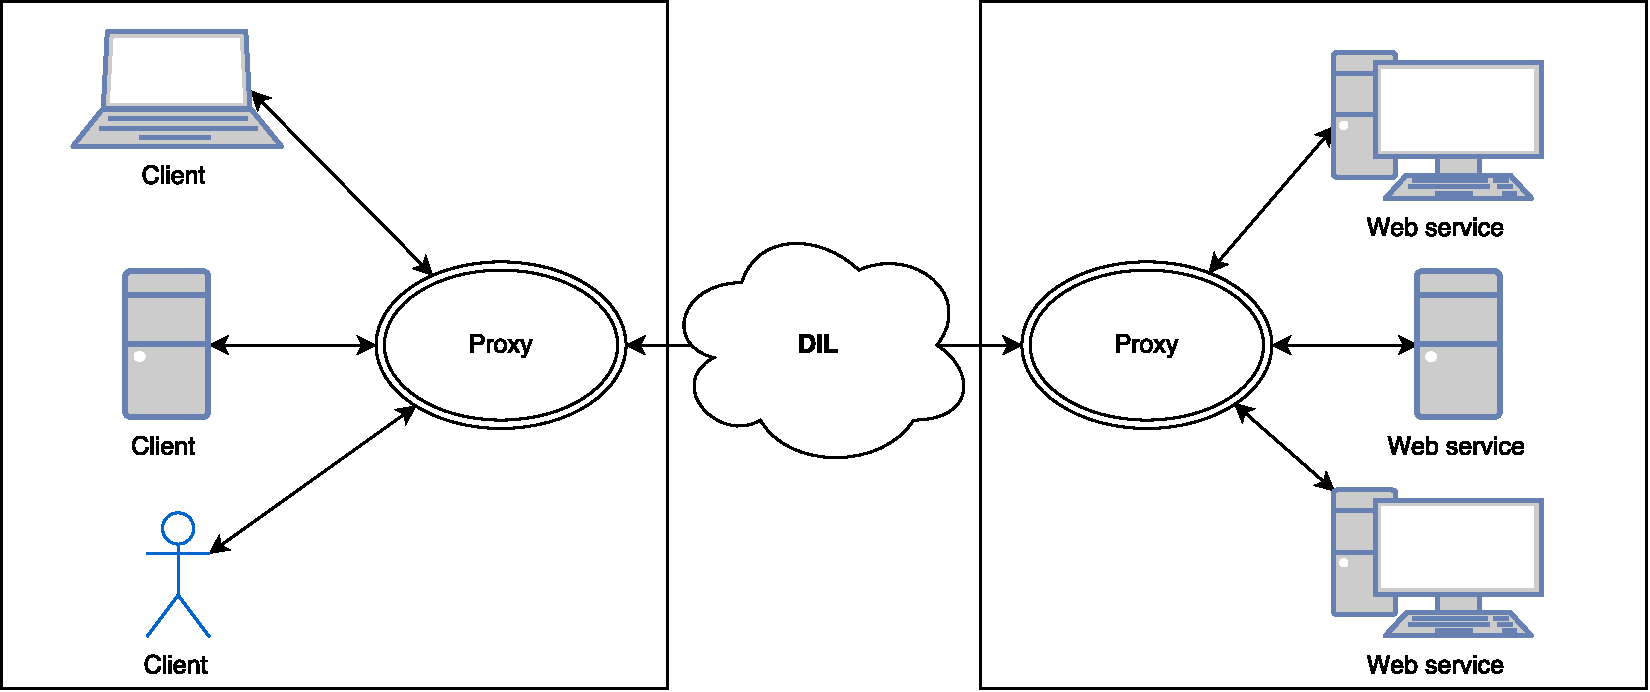
\includegraphics[scale=0.5]{images/proposed_solution.pdf}
\caption{Proposed proxy solution} \label{figure-proposed-proxy-solution}
\end{figure}


\subsection{Proxies}

A proxy is an application which acts as an intermediary between a client and a
server. Proxies are widely in use and their usage and type varies. Example of
proxy usage is for load balancing, caching and security. Web proxies are proxies
that forward \gls{http} requests, which is what we are investigating in this
thesis. This proxy will support features for compression, delay tolerance and
overcome network disruptions.


\section{Problem Statement}
Most of the Web service solutions used today are aimed for civilian use and do
not necessarily perform well in military environments. In contrast to civilian
networks where the date rate is abundant, mobile tactical networks may suffer
from high error rates and low date rate. Adapting Web service solutions meant
for civil networks directly for military purposes may not be possible.
Therefore, Web services needs to be adapted in order to handle network
challenges. However, it can be very expensive to alter existing Web service
technology and incorporate proprietary solutions. A NATO research task group has
previously identified the foundation on open standards to avoid tighter coupling
between service providers and consumers\cite{ist-090}. It is much better to use
\gls{cots} software. By placing the optimization in proxies, the
Web services can remain unchanged.

The goal of this thesis is to investigate different optimization techniques that
can be applied in order to improve Web service performance in \gls{dil}
networks. In order for the clients and services to remain interoperable the
optimization techniques will be placed in proxies. The Web services will
communicate as normal, while all network traffic is tunneled through a proxy.
The Web service itself does not need to pay attention to the bad connectivity,
the proxy will choose the appropriate protocol and configuration.

\section{Premises of thesis}

In this section we define the premises for the thesis and the proxy being
developed as a part of this thesis. As we have previously discussed, W3C Web
services are in widespread in use NATO, and the REST architectural style
has identified as a technology of interest to NATO. The first and second
premise is therefor that the proxies must support both REST and Web service
communication between machines connected in a DIL network. Next, in order to
optimize Web services in DIL environments, the applications themselves should
not be required to be customized, all optimization should be placed in proxies.
This retains the interoperability with standardized solutions(COTS). The forth
and final premise is that the proxy must work with standard security mechanisms.
In our case this means that any messages sent through the proxies, must be
exactly the same at the receiver as it would have been without the proxies. This
is due to both the header fields and the body of the message can be part of
security mechanisms, such as checksums and the presence of authentication header
fields.

To summarize, the premises of this thesis are listed here:

\begin{enumerate}
    \item Support RESTful and W3C Web services.
    \item Work in DIL networks.
    \item Interoperable with standardized solutions(COTS).
    \item Work with security mechanisms.
\end{enumerate}

\section{Scope and Limitations}

The goal of this thesis is to investigate optimization techniques for Web
services in \gls{dil} environments. We limit it to techniques that can be
applied at the application or the transport layer of the Internet protocol
suite(see \cref{figure-network-layers}). The reason for this is that NATO has
previously decided "everything over IP", a statement describing that all data
communication in NATO should occur with IP packets\cite{nnec-study}. We
therefore limit our optimization possibilities to the mentioned layers.

Since we focus on performance of Web services in this thesis, security is not
addressed. However, applications that are to be used in military
networks need to be approved by security authorities. If the application is too
complex, e.g. it has a very large code base or use a lot of external frameworks,
the approvement process can be very lengthy. It is therefore a important
consideration to make the proxy as relatively simple as possible.

Finally, the proxy implemented as a part of this thesis, only accepts \gls{http}
as input from the Web services. As we discuss later in \cref{web-services}, this
is a fair limitation since most Web services use \gls{http} to communicate with
other applications.


\section{Research Methodology}
Denning.


\section{Contribution}

The outcome of this thesis is a recommendation regarding which optimizations
techniques can be used in DIL to enhance the performance of Web services. As
well as a prototype implementation of a DIL proxy.

\section{Outline}
Hvordan er resten av oppgaven strukturert.
